\documentclass[11pt]{article}
\usepackage{geometry}                % See geometry.pdf to learn the layout options. There are lots.
\geometry{letterpaper}                   % ... or a4paper or a5paper or ... 
%\geometry{landscape}                % Activate for for rotated page geometry
%\usepackage[parfill]{parskip}    % Activate to begin paragraphs with an empty line rather than an indent
\usepackage{graphicx}
\usepackage{amssymb}
\usepackage{epstopdf}
\usepackage{hyperref}
\DeclareGraphicsRule{.tif}{png}{.png}{`convert #1 `dirname #1`/`basename #1 .tif`.png}

\title{DIO Cluster Study}

\begin{document}
\maketitle

\section{Abstract}

We did a a study of comparison of efficiency between inner radius of 39cm and 36cm. The result of this study may seem counter intuitive. But, it is actually very easy to understand. Let us start with the result of the study. We found that there is no loss in efficiency for moving the inner radius from 36cm to 39cm. The result is shown in figure \ref{fig:cluster_energy} The reason is because of the very hot region at the inner-front corner that cannot be used for any purpose if we want to get $<5\%$ resolution.
\begin{figure}[htbp]
   \centering
   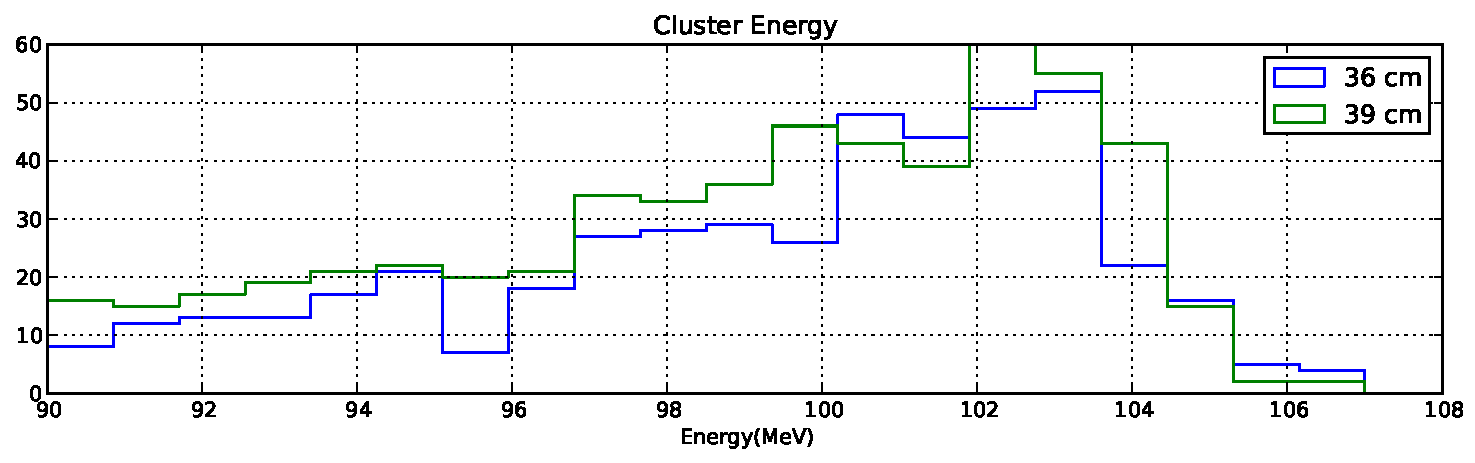
\includegraphics[width=\textwidth]{../plot/clusterenergy.pdf} % requires the graphicx package
   \caption{Total cluster energy for vanes with inner radius of 36cm and 39cm. The normalization here is the correct one because we did generate 1000 signal event at the target. The figure is zoomed to show qualitatively the resolution.}
   \label{fig:cluster_energy}
\end{figure}

\section{The Study}
\subsection{Exploring the Hitmap}
This study was done with Geant4 simulation written by Bertrand. It simulates DIO and signal hitting vanes or 12x44 (36cm) crystals and 11x44(39cm) crystals. We want to compare the efficiency and resolution of the two set of crystals. Intuitively, although not correct, we would expect to lose significant amount of efficiency in the smaller set of crystals. Latter section of the text will explain why this is not true. 

In this study, DIO and signal were generate track by track basis. We generated 1000 signal events for signal and 10000 events for background for both set of crystals. We only recorded ones that make a hit in the vane. The number of event we found for each set of crystal and for each type of event are shown in Table \ref{tab:numevent}. The relative number of signal is the correct normalization because we did generate 1000 event at the target with the full spectrum. However, the relative number of DIO is not meaningful because we are generating it out of a spectrum with different cutoff energy to save time. 

% Requires the booktabs if the memoir class is not being used
\begin{table}[htbp]
   \centering
   %\topcaption{Table captions are better up top} % requires the topcapt package
   \begin{tabular}{ lcr } % Column formatting, @{} suppresses leading/trailing space
		\hline
		Inner Radius & Signal & DIO\\
		\hline
      	36cm & 791 & 4618\\
		39cm & 798 & 2597\\
		\hline
      \end{tabular}
   \caption{Number of event for each type of sample and each set of crystals.}
   \label{tab:numevent}
\end{table}

For a signal event, we mixed up the DIO background by picking 27 DIO background and mix them up for the case of 36cm.  The number 27 is from 110/4 taken from page 6 of Giovanni's talk on 10/7/2011. For the 39cm, we only mix 2 DIO background per signal event. This number is from Bertrand's Geant4 simulation. Some samples of hits for each type of event are shown in appendix \ref{sec:typical_hit}.

The clustering algorithm is explained in detail in appendix \ref{sec:clustering_algorithm}. This section here will walk through the important part of the algorithm with the result that shows why we made some of the decisions. The first step of the clustering algorithm is to find the seed for the cluster. So, first let's take a look at the energy of the peak crystal shown in Figure \ref{fig:e_peak}. Note that this is from individual hit and not the pile up. From this figure, we decide to make an energy cutoff for the seed crystal at 50 MeV. 
\begin{figure}[htbp]
   \centering
   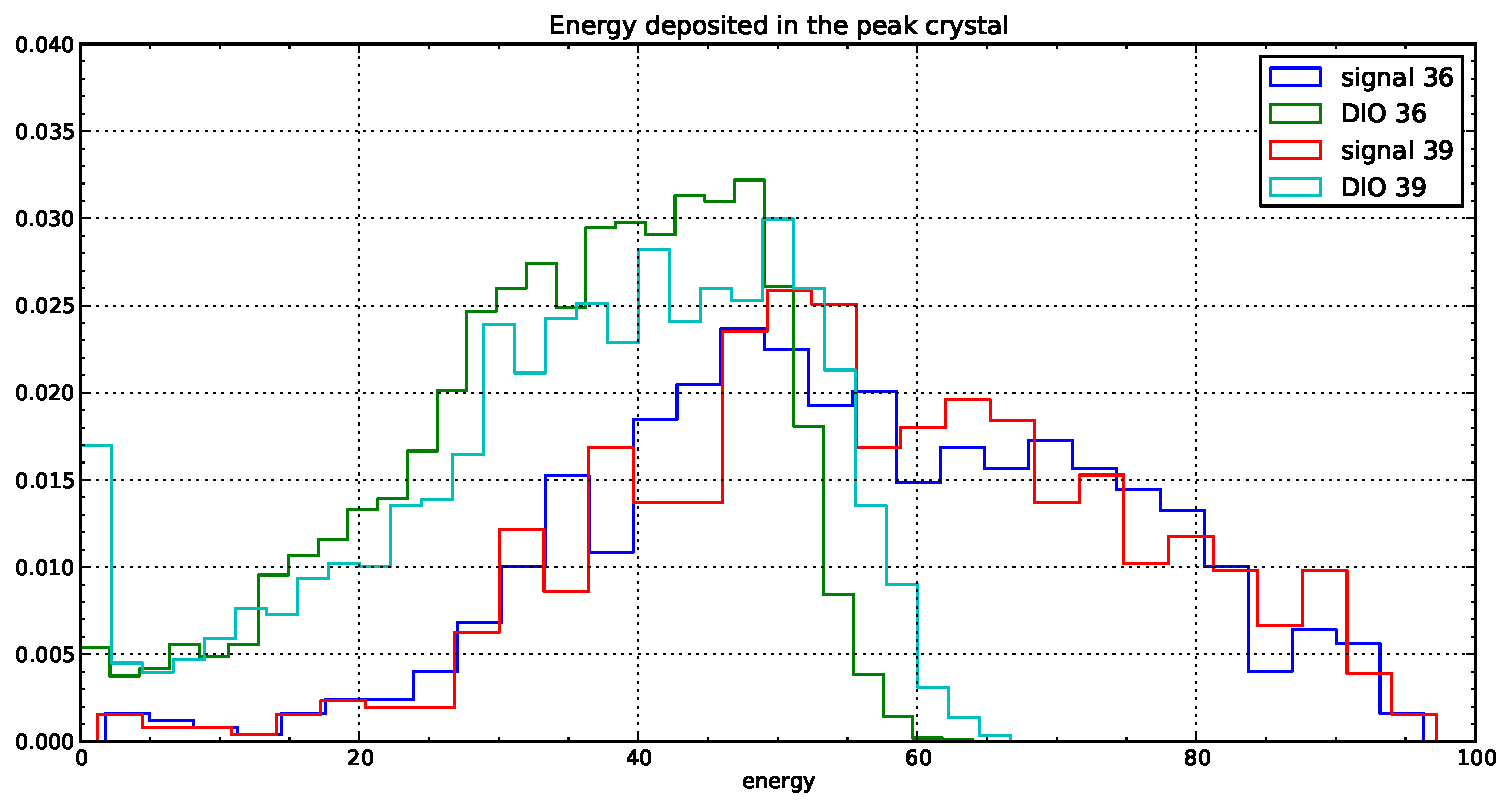
\includegraphics[width=\textwidth]{../plot/E_peak.pdf} % requires the graphicx package
   \caption{Energy deopsited in the peak crysal}
   \label{fig:e_peak}
\end{figure}

The location of the peak crystal are shown in Figure \ref{fig:sig_peak_loc_36},\ref{fig:dio_peak_loc_36}, \ref{fig:sig_peak_loc_39},\ref{fig:dio_peak_loc_39}. Note that the DIO used in these plots are individual hits not the pile up one. It is clear from this figure that we are going to have a lot of DIO pile up at the inner front region.

\begin{figure}[htbp]
   \centering
   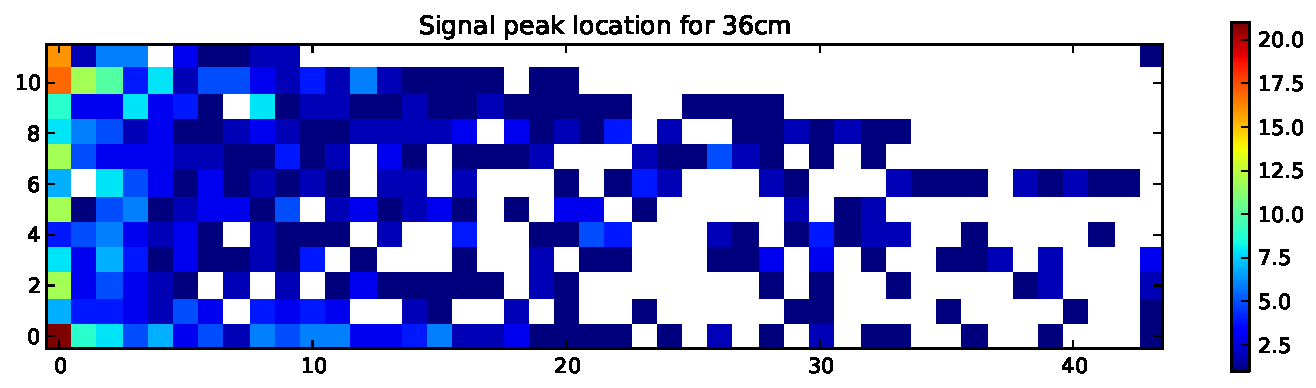
\includegraphics[width=\textwidth]{../plot/sig_peak_loc_36.pdf} % requires the graphicx package
   \caption{Location of the peak crystal from signal events for 36cm.}
   \label{fig:sig_peak_loc_36}
\end{figure}

\begin{figure}[htbp]
   \centering
   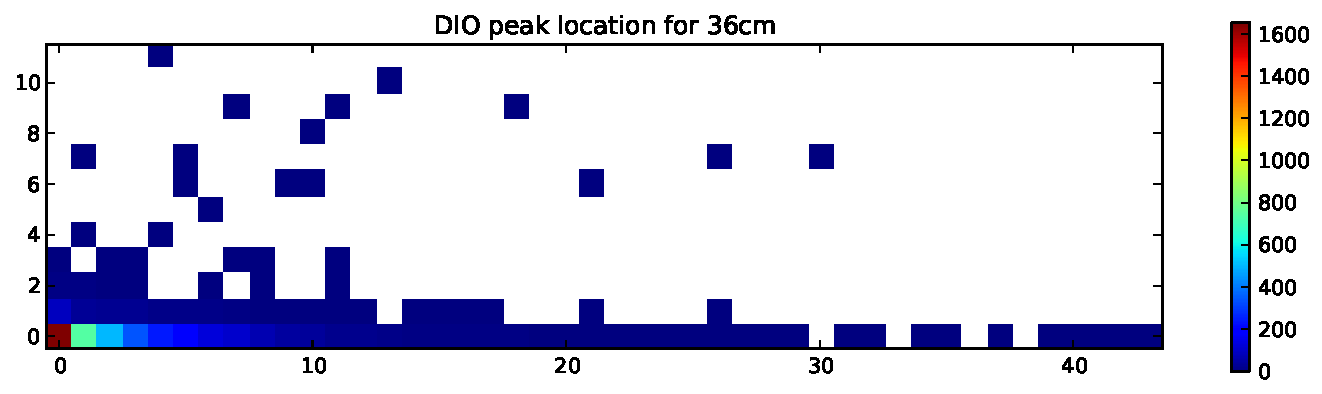
\includegraphics[width=\textwidth]{../plot/dio_peak_loc_36.pdf} % requires the graphicx package
   \caption{Location of the peak crystal from DIO events for 36cm.}
   \label{fig:dio_peak_loc_36}
\end{figure}

\begin{figure}[htbp]
   \centering
   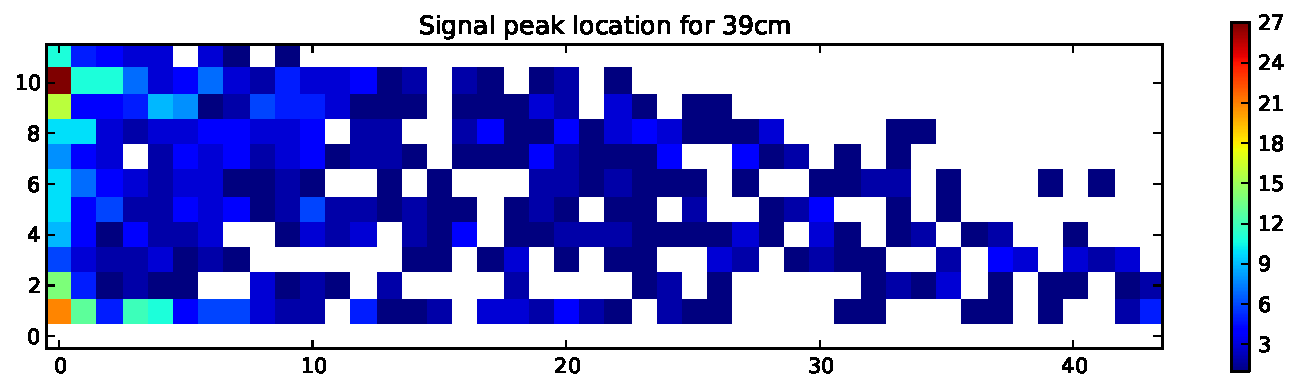
\includegraphics[width=\textwidth]{../plot/sig_peak_loc_39.pdf} % requires the graphicx package
   \caption{Location of the peak crystal from signal events for 39cm.}
   \label{fig:sig_peak_loc_39}
\end{figure}

\begin{figure}[htbp]
   \centering
   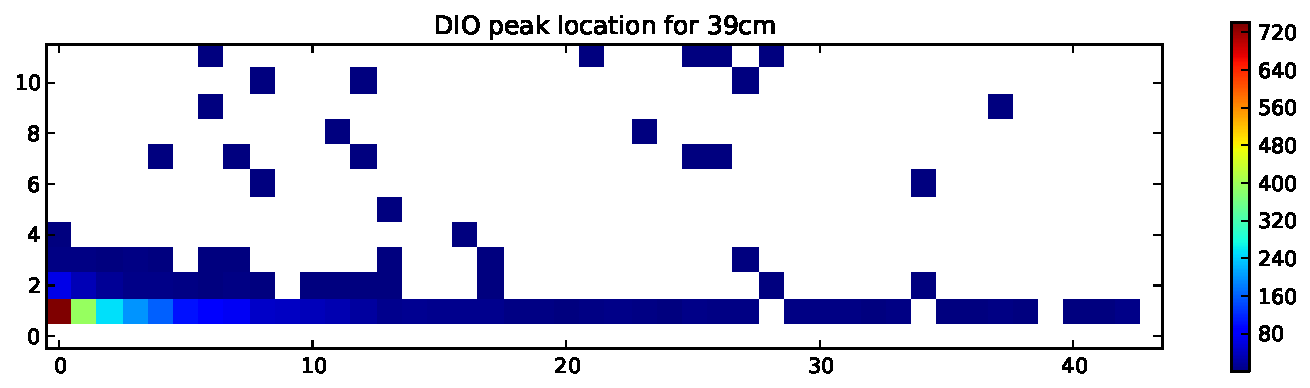
\includegraphics[width=\textwidth]{../plot/dio_peak_loc_39.pdf} % requires the graphicx package
   \caption{Location of the peak crystal from DIO events for 39cm.}
   \label{fig:dio_peak_loc_39}
\end{figure}

We, therefore, looked at the average energy of pile up DIO hits [\ref{fig:average_dio_hit_36},\ref{fig:average_dio_hit_39}] and found that the inner front corner crystal has too much pile up for any energy measurement purpose. The 0,0 crystal has 340MeV inside. If we want to get a 5\% resolution for the signal electron, we need to cut out crystals that has more than 5MeV inside on average. These crystals are called hot regions and are removed from clustering. These crystals are shown in figure \ref{fig:removed_crystals}.
\
\begin{figure}[htbp]
   \centering
   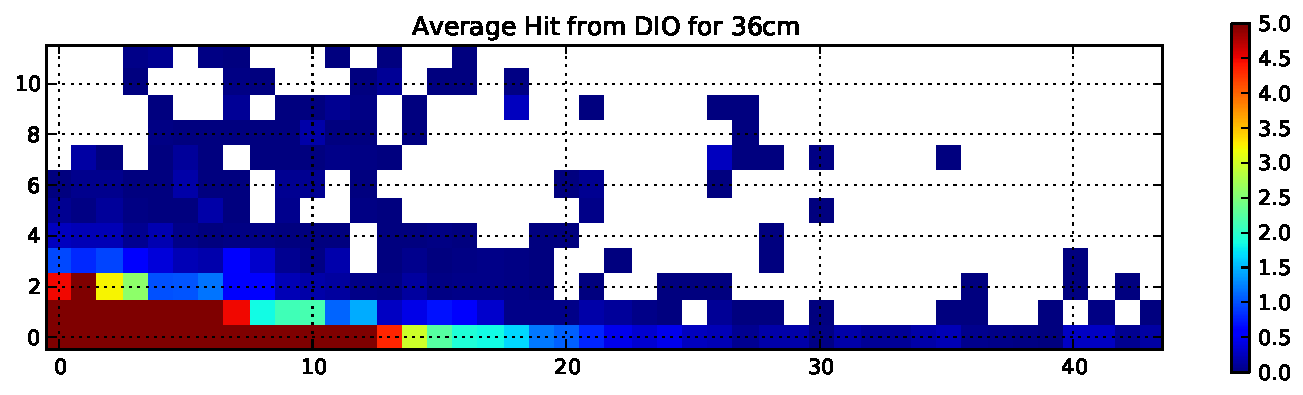
\includegraphics[width=\textwidth]{../plot/average_dio_hit_36.pdf} % requires the graphicx package
   \caption{Average DIO energy deposited in each crystal for 36cm.}
   \label{fig:average_dio_hit_36}
\end{figure}

\begin{figure}[htbp]
   \centering
   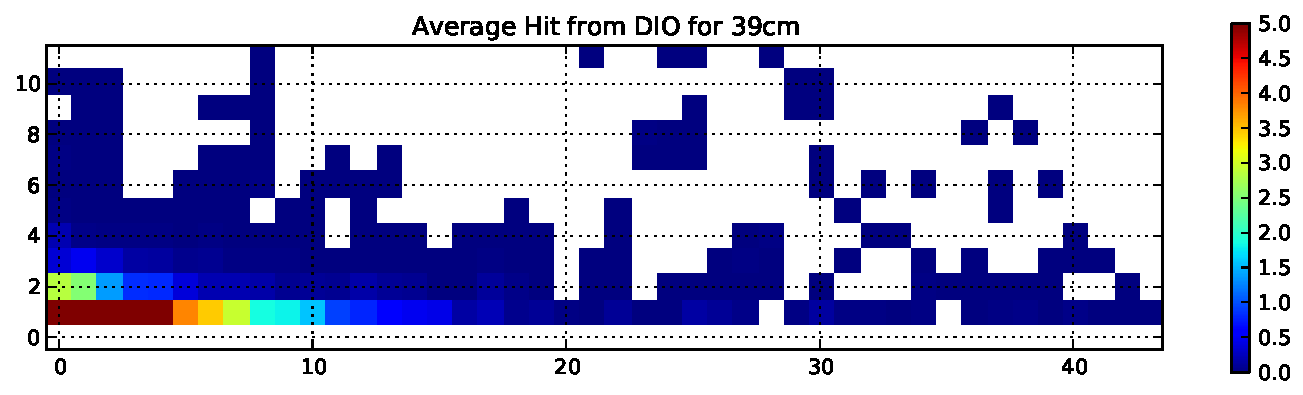
\includegraphics[width=\textwidth]{../plot/average_dio_hit_39.pdf} % requires the graphicx package
   \caption{Average DIO energy deposited in each crystal for 39cm.}
   \label{fig:average_dio_hit_39}
\end{figure}

\begin{figure}[htbp]
   \centering
   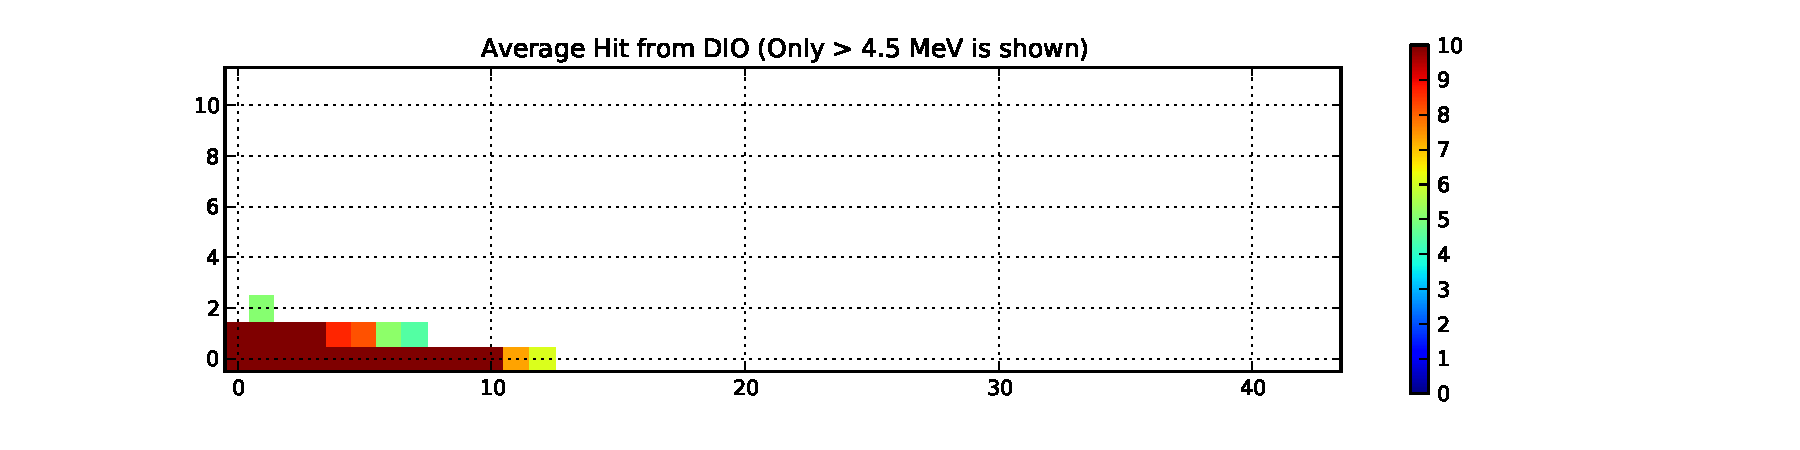
\includegraphics[width=\textwidth]{../plot/removed_crystals.pdf} % requires the graphicx package
   \caption{Crystals that have energy more than 4.5MeV. We remove these crystals from the clustering algorithm}
   \label{fig:removed_crystals}
\end{figure}
\clearpage

\subsection{Clustering Result}
From the previous section, we justify the choice for ignoring the hot regions and the seed energy cut at 50MeV. We did clustering for both inner radii. The cluster energy is plotted in Figure \ref{fig:cluster_energy} and \ref{fig:cluster_energy_no_zoom}. Note that the normalization for both of them can be compared on 1:1 based. Note that the high tail comes from the signal cluster eating close into shower from hot region. To compare the efficiency, we count number of clusters we found that has energy between 96 and 105MeV. We found 359 and 415 clusters for 36cm and 39cm accordingly. It is quite clear from \ref{fig:cluster_energy_no_zoom} that 39cm is the better choice. 

\begin{figure}[htbp]
   \centering
   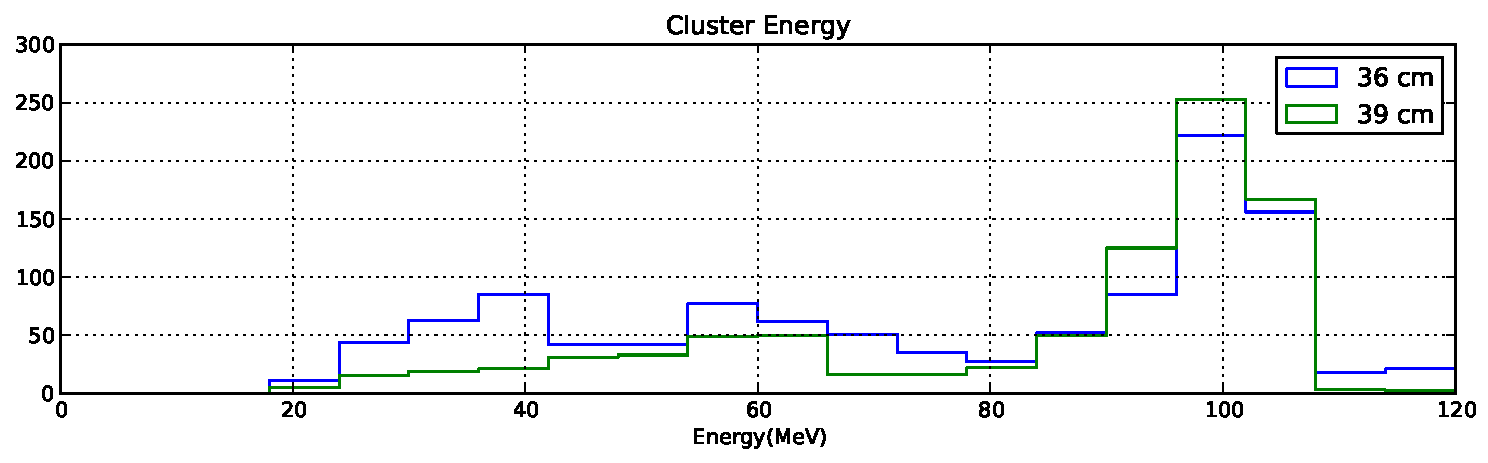
\includegraphics[width=\textwidth]{../plot/clusterenergy_no_zoom.pdf} % requires the graphicx package
   \caption{Total cluster energy for vanes with inner radius of 36cm and 39cm. The normalization here is the correct one because we did generate 1000 signal event at the target. The figure is zoomed to show qualitatively the resolution.}
   \label{fig:cluster_energy_no_zoom}
\end{figure}

\subsection{Some Discussion on Hot Region}

The reason that 39cm inner radius is the signal will manage to hit the next row in the next vane but background could do the same thing due to low $p_z$. The background at 50ish MeV have a very small energy budget. It needs a large $p_T$ to have radius barely large enough to hit a vane. Therefore, it has very small energy in $z$ direction which make it's pitch really small. Therefore, when we remove the first row, it will rarely go on and hit another vane at higher column. However, the signal has 100 ish MeV of energy budget. Even with large $\cos \theta$ it will have a large radius and large pitch. It just happen to be unlucky to hit the first row.

We could take advantage of the small pitch nature of the DIO background to put a shielding material near the target at low $\cos \theta$. But, this may produce a bunch of track inside the tracker.

With disk detector We will most likely see the same effect but at a smaller magnitude since there aren't that many column as in vane detector. 
\clearpage
\appendix
\section{Clustering Algorithm}
\label{sec:clustering_algorithm}
Our clustering algorithm is a simple one which has basically 3 step: find seeds, expand the seeds into clusters and split the clusters.
\begin{enumerate}
\item In this implementation we find the seed, with a simple energy cut. We look for crystals in non-hot region[\ref{fig:removed_crystals}] with energy more than 50MeV.
\item We then sort the seed list by energy.
\item Pop the highest energy seed from the list. Then, recursively expand the seed looking for crystals within a 3x3+4 diamond shape area that has energy more than 1\% of the seed crystal. Crystals in hot-region are completely ignore. If the cluster expand into another seed in the seed list, we remove that seed from the seed list.
\item Repeat 2 until the seed list is empty. After the list is empty, we got a list of clusters.
\item For all crystals that are in two or more clusters, we calculated the "expected" energy using gaussian with width of moire radius with peak normalized to the peak crystal using the distance from the peak crystal to the overlapped crystal. The crystal is then given to the cluster with the highest "expected" energy. This step is very rare in this study. 
\end{enumerate}
\clearpage
\section{Some typical hits}
\label{sec:typical_hit}

\begin{figure}[htbp]
   \centering
   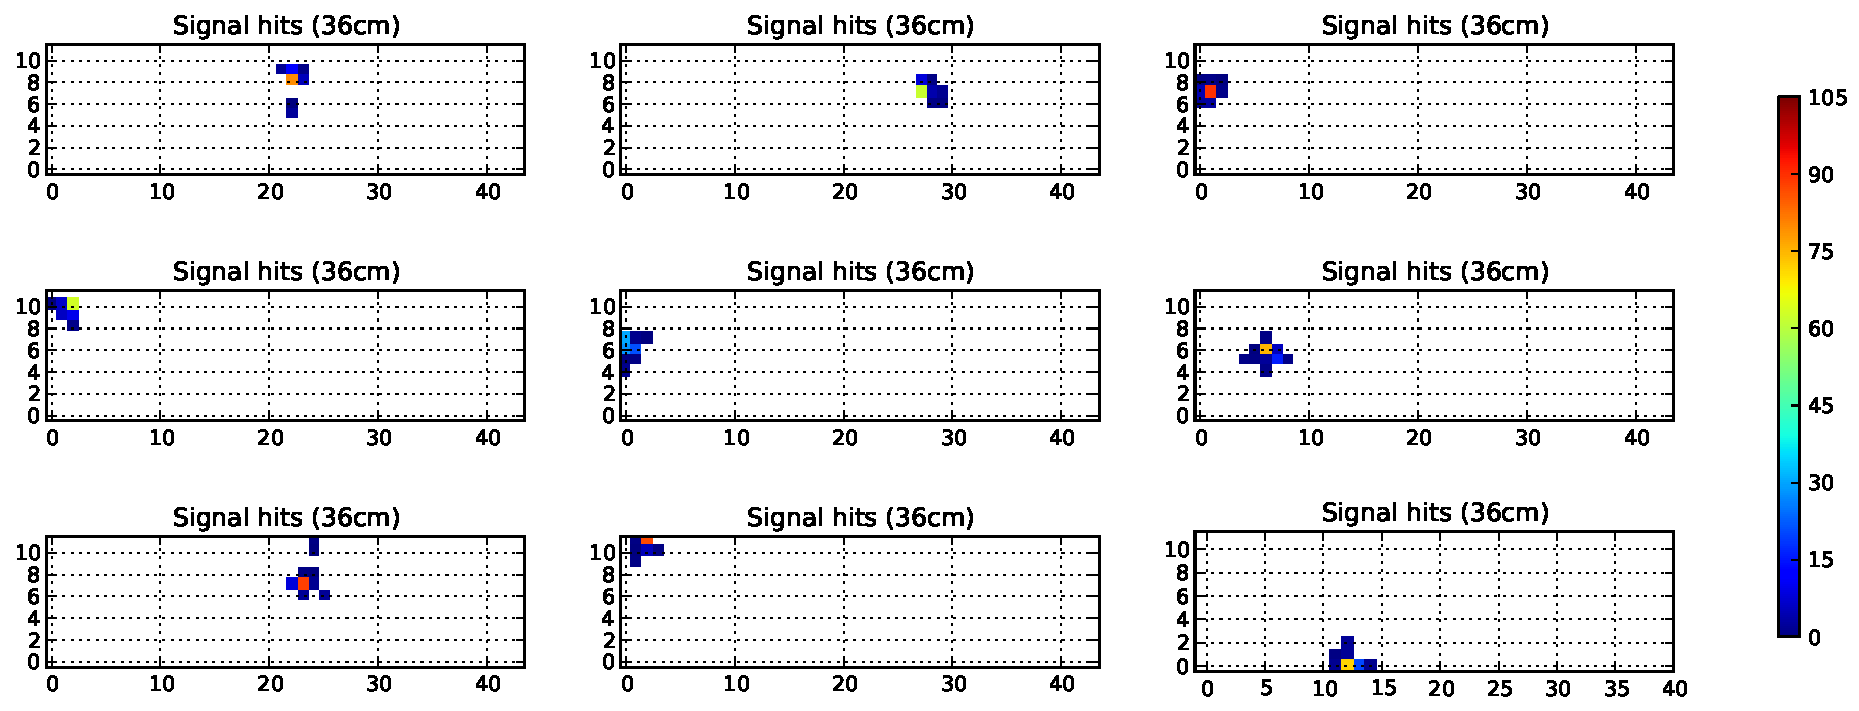
\includegraphics[width=\textwidth]{../plot/sig_sample_hit_36.pdf} % requires the graphicx package
   \caption{Some sample of signal hit for 36 cm}
   \label{fig:sig_sample_hit_36}
\end{figure}

\begin{figure}[htbp]
   \centering
   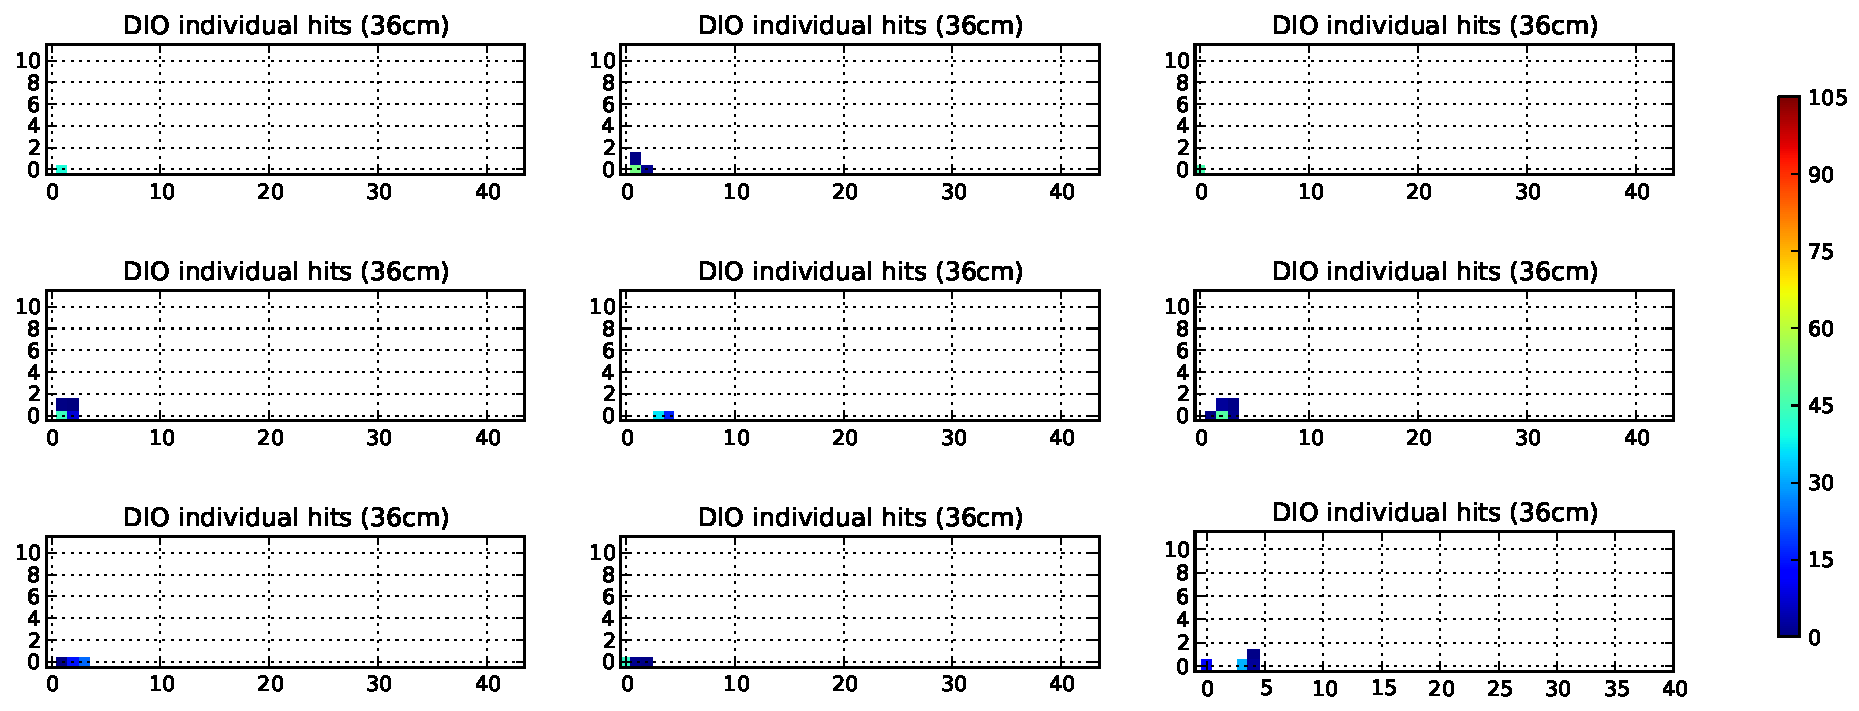
\includegraphics[width=\textwidth]{../plot/dio_sample_hit_36.pdf} % requires the graphicx package
   \caption{Some sample of individual DIO hit for 36 cm}
   \label{fig:dio_sample_hit_36}
\end{figure}

\begin{figure}[htbp]
   \centering
   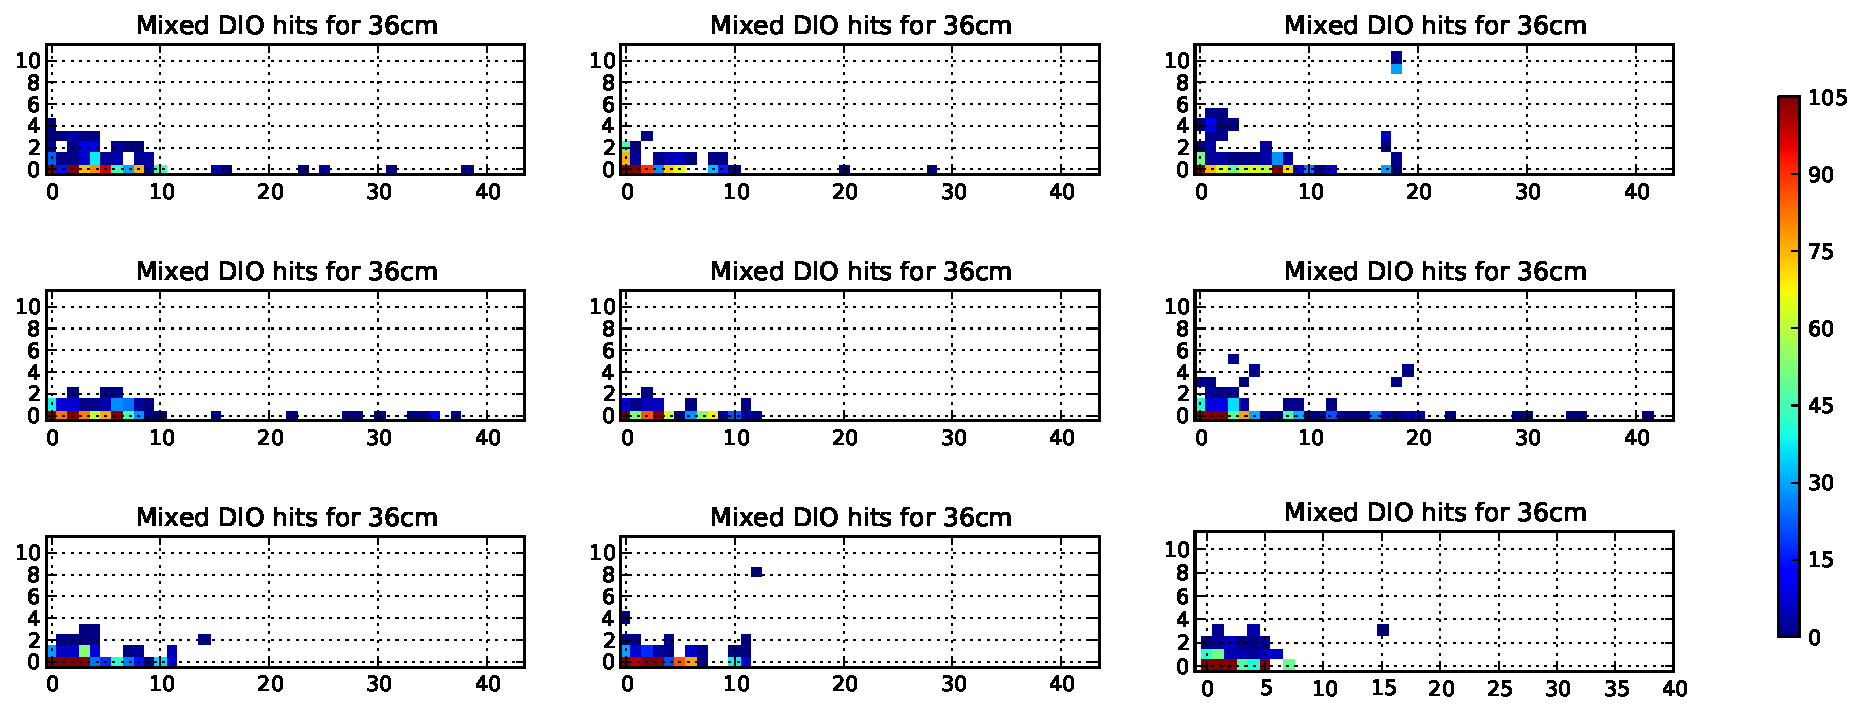
\includegraphics[width=\textwidth]{../plot/mixed_dio_sample_hit_36.pdf} % requires the graphicx package
   \caption{Some sample of mixed DIO hit for 36 cm}
   \label{fig:mixed_dio_sample_hit_36}
\end{figure}

\begin{figure}[htbp]
   \centering
   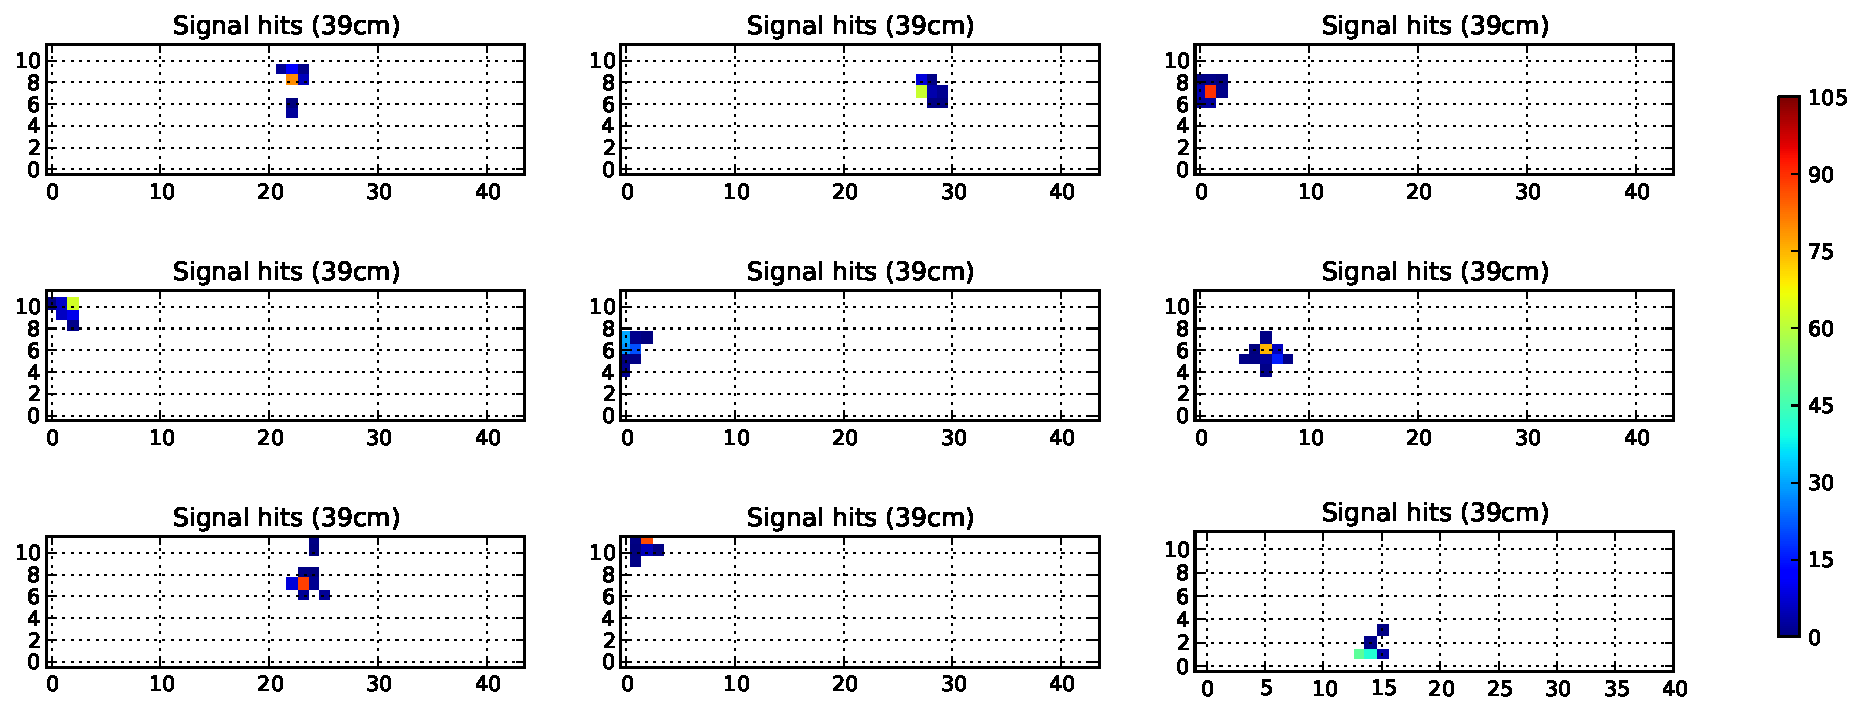
\includegraphics[width=\textwidth]{../plot/sig_sample_hit_39.pdf} % requires the graphicx package
   \caption{Some sample of signal hit for 39 cm}
   \label{fig:sig_sample_hit_39}
\end{figure}

\begin{figure}[htbp]
   \centering
   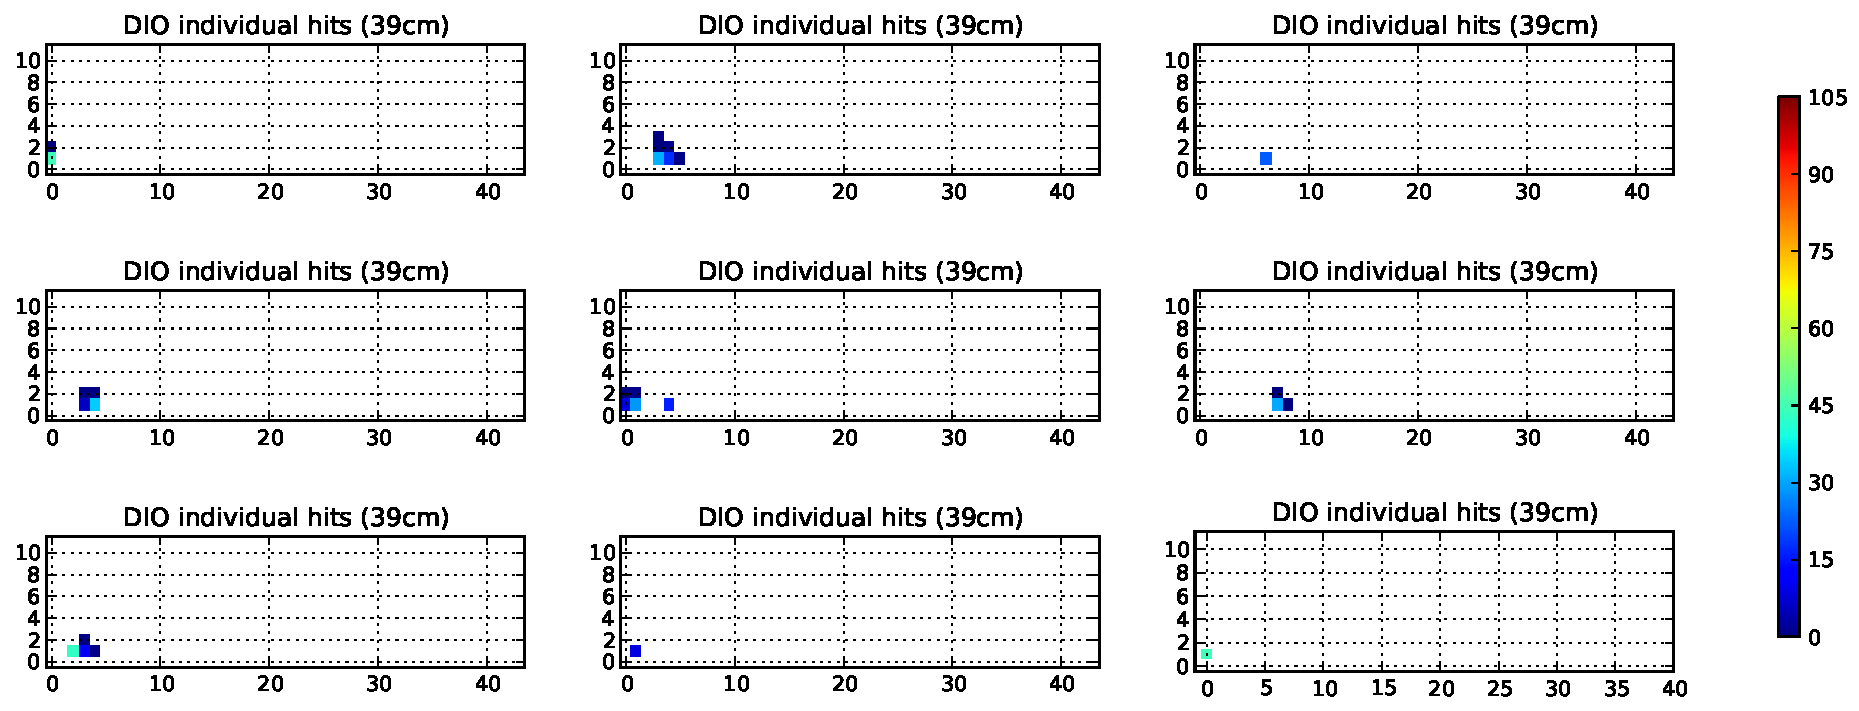
\includegraphics[width=\textwidth]{../plot/dio_sample_hit_39.pdf} % requires the graphicx package
   \caption{Some sample of individual DIO hit for 39 cm}
   \label{fig:dio_sample_hit_39}
\end{figure}

\begin{figure}[htbp]
   \centering
   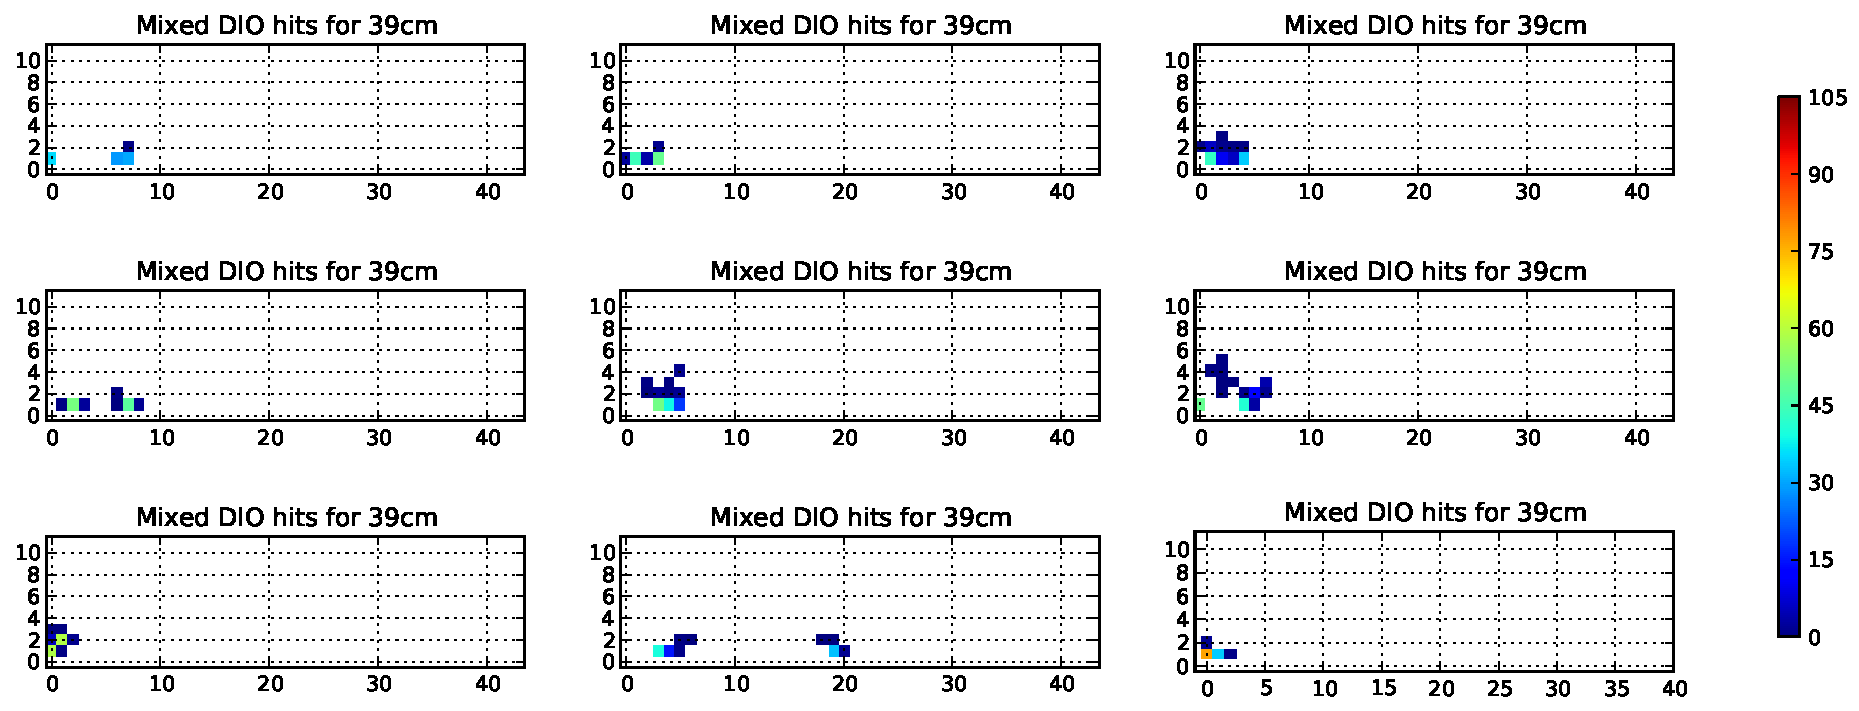
\includegraphics[width=\textwidth]{../plot/mixed_dio_sample_hit_39.pdf} % requires the graphicx package
   \caption{Some sample of mixed DIO hit for 39 cm}
   \label{fig:mixed_dio_sample_hit_39}
\end{figure}


\end{document}  